\label{ch:res}
%In the previous chapters, many different methods that can be used to compute PESs numerically are described and in chapter \ref{ch:proced} the method used within this work is described in more detail.
%In this chapter some results are shown and explained.
Since the method developed in this work combines several techniques that have not been used together so far and quantum-mechanical continuum-function are not treated with the infinite elements technique so far, several conceptual questions need to be clarified before computing actual PESs.
In section \ref{ch:BCbench}, infinite elements are compared with Dirichlet BCs and their respective influence on the properties of the wave function is studied. %In section \ref{sec:NumConve} further benchmarking calculations on some numerical parameters are shown.
These calculations are performed using atomic lithium and hydrogen as test system.
Especially the case of hydrogen is of interest here since analytic solutions to compare with are available.
Thereafter, in section \ref{sec:cs}, the energy-dependence of the cross section for the valence transition of lithium as well as several transitions of carbondioxide are studied, comparing several theoretical approaches with experimental data.
Moreover, the PESs of CO$_2$ and benzene as computed with several theoretical approaches are shown.

\section{Comparison of Boundary Conditions}
\label{ch:BCbench}
In section \ref{ch:BC}, several BCs which give rise to different properties for the solution have been briefly overvied.
Detailed studies on absorbing BCs, non-reflecting BCs as well as complex absorbing potentials can be found in literature \cite{babuska,artBC,capComp,absRev,nrBCrev}.
In this work, Dirichlet boundaries and infinite elements are studied in more detail and the properties of the respective results are compared.
Even though the validity of Dirichlet BCs is questionable for unbound problems, they are easy to apply and their physical consequences provide quite straightforward interpretation of the results.
Thus, they provide a good comparison for the study of infinite elements, whose properties are not studied in this context yet.
The infinite elements are the main objective of this work.
Since they provide a reasonable description for outgoing particles, they allow for a small simulation region, even if the wavelength is very large.
Moreover, they have the correct asymptotic behaviour and hence are expected to produce a good representation of continuum solutions.
In section \ref{sec:DBCbench}, systematic tests are made, studying the dependence of the eigenenergies as well as the properties of the wave function on the parameters of the numerical grid used.
Thereafter, in section \ref{sec:iBCbench}, further tests with infinite elements show the influence of these boundary conditions on the solution.
%First, in section \ref{sec:DBCbench} several properties of the grids introduced in section \ref{sec:grid} are studied with Dirichlet boundaries which are particularly easy to set up and understand in their physical consequences provide straightforward interpretation of the results.
%In section \ref{sec:iBCbench}, several properties of the mesh with infinite elements are investigated.
Since it turns out that the solutions obtained with infinite elements are very sensitive to the parameters of mesh and simulation box, this study is performed more extensively.
%For simplicity, the tests shown here are on atomic systems using, unless specified otherwise, an analytic Coulomb potential with charge $1$, corresponding to the ionised hydrogen atom.


\subsection{Dirichlet Boundary Condition}
\label{sec:DBCbench}
Dirichlet boundaries are conceptually the easiest BCs but are known to have a large influence on the solution, especially for continuous functions since they reflect outgoing waves fully.
%\begin{wrapfigure}{l}{0.6\textwidth}
%\includegraphics[width=0.6\textwidth]{Figures/BC/DBCenergies}
%\caption{double-logarithmic plot of the error in energy of the energetically closest solutions in dependence on the radius
%of the sphere. The comparison with $\propto \frac{1}{r^3}$ shows the general behaviour of the error.}
%\label{fig:dbcRad}
%\end{wrapfigure}
\begin{figure}
\includegraphics[width=\textwidth]{Figures/BC/DirichletBC}
\caption{Results obtained with Dirichlet BCs using different box sizes:
a) double-logarithmic plot from the deviation in energy for the solutions closest to the target energy $E_\text{target}=0.566\,$Hartree as a function of the radius of the simulation box;
b) real part of $d$-wave functions obtained with different boxes ($r_\text{max}=4\,$bohr and number of spheres $N=18$, blue line and $r_\text{max}=10\,$bohr and $N=38$ spheres, red line); Coulomb wave (yellow line) is also presented for comparison;
c) and d) show the deviation in energy for box radii of $4\,$ and $10\,$bohr,\ varying the number of spheres (radial grid density, see \eq{eq:tm_map}) in the box;
e) and f) show the partial wave contributions \eq{eq:PartWaveCoeff} having different angular momenta for the the respective solutions with $r_\text{max}=4$ and $N=16$ (left) as well as $r_\text{max}=10$ and $N=38$, respectively.}
\label{fig:dbcRad}
\end{figure}
Moreover, its requirement for the solutions to vanish at the boundaries results in an artificial discretisation of the spectrum similar to that of bound states.
This leads to a banded spectrum, with the energy gap between two states being dependent on the simulation box size.
%Moreover, these boundaries enforce the real and imaginary part of the solution to be identical up to a scaling operations (such as rotations and reflections for spherical systems) which does not hold for continuum waves such as Coulomb waves as can be seen in Figure \ref{fig:RadFun} and plane waves that have a constant phase shift.

%These properties are found in various tests conducted to find reasonable parameters for application to more complex systems.
To understand the general properties of solutions for Dirichlet BC and to formulate requirements to the mesh quality, the method has been first tested on the hydrogen-like system with $\nicefrac{1}{r}$ ESP.
To do so, the radius of the simulation box $r_\text{max}$ and the number of spheres, $N$, see \eq{eq:tm_map} has been varied to get convergent results.
In Figure \ref{fig:dbcRad} a), the deviation in the energy of $15$ solutions is shown for different $r_\text{max}$ (see \eq{eq:tm_map}), the number of spheres is kept constant at $N=20$.
The comparison with the red line that represents a $\nicefrac{\text{const}}{r^3}$ dependence, shows that the error is inverse proportional to the volume of the box which is a well-known result for particles in a box with infinite potential walls. 
The number of spheres is kept constant at $N=20$.
The influence of radial grid density on the energies is shown in the panels c) and d) of Figure \ref{fig:dbcRad} where the number of spheres is varied for two different box-sizes, $r_\text{max}=4$ and $r_\text{max}=10\,$bohr, respectively.
In these figures several branches of solutions can be seen that correspond to different angular momenta.
For smaller radii ($r_\text{max}=4\,$bohr, panel c)), these branches are well-separated but become closer and interfere with each other at larger radii ($r_\text{max}=10\,$bohr, panel d)).
Following the expectations, the energies of the respective branches decay when the number of grid points.
At $N=18$ for $r_\text{max}=4\,$bohr the results converge and do not change much with further increase of $N$.
However, for $r_\text{max}=10\,$bohr the convergence is much slower and cannot be reached for $N<60$.
In principle, the continuum spectrum should have infinite degeneracy containing FEFs corresponding to arbitrary angular momenta and since larger boxes provide higher density of states it may be considered desirable to take as large simulation boxes as possible.
This in general also agrees with the common logic for quantum mechanical calculations.
However, the density of states is not the only important quantity: The PES intensities beinge the main objective in the present work are calculated using the DO.
Due to the aufbau principle, usually the atomic states with quite low angular momentum are populated.
\textit{E.g.} in molecules and atoms consisting of second period elements one can expect only $s$ and $p$ atomic functionals to be populated in the lowest excited electronic states. 
Thus, one can expect that FEFs only up to $l=2$ could contribute to PES intensities if the dipole selection rules hold.
That is why to reproduce reliable intensities, the computational scheme should favour solutions with low angular momentum.

The panels e) and f) of Figure \ref{fig:dbcRad} show the projections of the solutions to the spherical wave functions with respective kinetic energy and different angular momentum, where the partial wave contribution is defined as
\begin{equation} \label{eq:PartWaveCoeff}
\sum_m|\langle \Psi_\text{n} | \Psi_{\vec{k},l,m}^\text{Sph}\rangle |^2.
\end{equation}
Here $|\Psi_{\vec{k},l,m}^\text{Sph}\rangle$ is the spherical wave \eq{eq:spherWave} with angular momentum $l$ and its projection onto the quantisation axis $m$ and $|\Psi_\text{n}\rangle$ denotes the respective numerically obtained solution.
The comparison is done against the spherical waves and not against Coulomb waves, since confluent hypergeometric functions are difficult to converge for larger $r$ and they are much more computationally demanding.

The testcalculations have shown that for the given energy of the photoelectron of $E=0.566\,$ Hartree the obtained solutions have a well-defined angular momentum only for small boxes where the critical radius is in the order of $r_\text{max}=10\,$bohr.
For larger computational domains, the states are mixed and have large contributions from much higher angular momenta and are very sensitive to different parameters such as the number of spheres $N_i$ and the parameters $s$ and $q$ in  \eqs{eq:tm_map} and (\ref{eq:son_map}) respectively.
Moreover, for example the comparison of the Figures \ref{fig:dbcRad} e) and f) shows that solutions with larger boxes tend to have higher angular momenta which is an important argument in favour of smaller boxes since for most atomic systems angular momenta larger than $4$ are not of interest for practical calculations.
This tendencey can be understood when considering the radial SE \cite{Lifshitz}
\begin{equation}
\frac{\partial^2}{\partial r^2} R(r) + \left(2\left(E-V(r)\right) -\frac{l(l+1)}{r^2}\right) R(r)=0
\end{equation}
where $R(r)$ is the radial solution and $E-V(r)$ is identified as kinetic energy.
Thus, given a particular kinetic energy, the radial oscillations are reduced by a larger angular momentum.
This leads to the interpretation that a particle can `distribute' its kinetic energy between the radial (outgoing) and spherical contributions.
In turn, however, needs a wave with large angular momentum more space and thus these solutions are suppressed in smaller computational domains.

In Figure \ref{fig:dbcRad} b), two solutions with $l=2$ along one axis are shown (the fifth one for $r=4$ and the first one for $r=10$ which are shown in \ref{fig:dbcRad} e) and f) as well) for two different box-sizes and compared to the Coulomb wave, being the exact solution for the $-\nicefrac{1}{r}$ potential.
As one can see, depends the reproducability of the radial structure strongly on the size of the box.

%\subsection{Complex Absorbing Potential}
%Using a CAP as described in section \ref{ch:cap}, two additional degrees of freedom comared to the Dirichlet BCs arise: the strength $\eta$ of the artificial potential (\ref{eq:cap}) and the offset $r_0$ where it starts, the latter has the only restriction to be larger than the radius of the DO.
%In section \ref{ch:cap} it was suggested to chose the parameters such that the respective derivatives of the energy vanish \cite{CAPccEOM,CAPfreshlook}.
%This procedure is, however, only valid if one solution should be taken into account and thus is not directly applicable here.
%Interpreting the real part of the eigenvalues of the eigenproblem (\ref{eq:SEmat}) as the energy of the respective state, the influence of the CAP on the density of states varies strongly when changing other parameters.

\subsection{Infinite Elements}
\label{sec:iBCbench}
The method making use of infinite elements has more different parameters which can be crucial for the stability of the solution than the Dirichlet BC.
Investigations of these dependences is the subject of the present section.


\begin{figure}%{R}{0.5\textwidth}
\begin{subfigure}{0.5\textwidth}
   \includegraphics[width=\textwidth]{Figures/BC/plane_fin}
   \caption{2D-cut of a solution with infinite elemnts using a spherical finite element region indicated by the red circle with a radius of $r=6\,$bohr and $N=11$ spheres.}
\end{subfigure}
\begin{subfigure}{0.5\textwidth}
   \includegraphics[width=\textwidth]{Figures/RBF/P-Wave}
   \includegraphics[width=\textwidth]{Figures/RBF/p_wave}
   \caption{$r_\text{max}=12.39$, $N=18$, scheme: tm, $s=2.5$, $q=1.2$}
   \label{fig:cutInf}
\end{subfigure}
%\caption{}
\end{figure}
In Figure \ref{fig:cutInf}, a 2D-cut of a solution obtained with infinite elements for the Hydrogen atom is shown, the red circle indicates the region of finite elements.
The features shown in Figure \ref{fig:cutInf} are prototypic for the properties that are found for the infinite elements here.
It is clearly visible from the graph that the infinite region resembles the asymtotic behaviour, showing the expected regular oscillations of an outgoing wave.
However, the angular momentum is quite large, leading to only small contributions in the finite element region.

%\subsubsection{Formulation of Infinite Elements}
\subsubsection{Comparison of Formulations}
\label{ch:bmFormul}
Before having a closer look at the convergence of different parameters, first the formulation of infinite elements to be used later is investigated.
Since the unconjugated Bur\-nett-formulation was not very successful \cite{dreyer}, the conjugated formulations of Burnett and Astley-Leis both have interesting features to use for quantum mechanical problems.
Since the conjugated Burnett elements lead to infinitely large matrix elements, here the Astley-Leis elements (\ref{eq:ALelem}) are compared with the symmetrised form (\ref{eq:ALsymm}) using different powers $p$.
Moreover, to study the influence of the damping function in the Astley-Leis formulation (\ref{eq:ALelem}) in more detail, also a test function space similar to eq. (\ref{eq:ALelem}) but using the squared damping function $D(r)^2$ instead of $D(r)$.

The 50 real solutions whose energy is closest to the target value of $15.44\,$eV ($0.5675\,E_h$) obtained with the original Astley-Leis formulations with the damping function taken to the powers $p=1,2$ as well as the symmetrised formulation (\ref{eq:ALsymm}) suggested in this thesis with powers $p<0.5$ are shown in Figure \ref{fig:IFEMform_spect}.
For the unsymmetric formulations only the real part is shown which is assigned to the physical energy of the respective state.
\begin{figure}
\includegraphics[width=\textwidth]{Figures/IFem_form_spectra}
\caption{The first 50 eigenvalues obtained with the original Astley-Leis formulation (imaginary part not shown) and with the symmetrised form \eq{eq:ALsymm}.}
\label{fig:IFEMform_spect}
\end{figure}
The results shown in Figure \ref{fig:IFEMform_spect} show clearly that the obtained density of states decreases with the power $p$ and converges for $p\approx \frac 18$ for the given parameters (the radial mapping scheme (\ref{eq:tm_map}) is used with $N=25$, $l=0.5$, $p=2.5$ and $r_\text{max}=7\,$bohr.).

The dependence of the obtained spectrum of the Hamiltonian on the power of the damping function shows that, at least for FEFs, the asymptotic behaviour is crucial for the properties of the wave function. 
The dependence converges for $p=1/8$, see also Figure \ref{fig:powerSpect} in supplement.
Moreover, even for small powers $p\approx 10^{-4}$, no numerical instabilities are observable so that there is some freedom in this parameter and it does not need to be optimised for different systems individually.
The observations made on the convergence-properties using the spectrum in Figure \ref{fig:IFEMform_spect} are supported by the projections of the solutions on spherical waves of which some are shown in Figure \ref{fig:IFEMform_project}.

\begin{figure}
\includegraphics[width=\textwidth]{Figures/Ifem_forms}
\caption{Decomposition of the first 30 solutions into spherical waves with angular momenta up to $l=7$.
Left: Astley-Leis-formulation ($p=1$), middle: symmetrised form ($p=0.5$) right: symmetrised form ($p=10^{-4}$).}
\label{fig:IFEMform_project}
\end{figure}

As shown in the Figure \ref{fig:IFEMform_project}, the nature of the states obtained is in all cases strongly mixed in the quantum number $l$ with significant contributions even for $l>7$.
However, the relative contributions of the angular momenta critically depends on the power $p$, making a reasonable choice of this parameter important.
Further it is expected that the convergence of $p$ depends on further parameters such as the box-size and kinetic energy of the photoelectron which is, however, not studied here in more detail.
Instead, in the following the power of the damping function $D$ is chosen to be $p=0.0001$ if not specified differently.
This value is far in the convergence region of Figure \ref{fig:IFEMform_project} and thus is hoped to be reasonable also for other systems.

%\subsection{Size of Finite Element Region}
\subsubsection{Radius of the Finite Element Region}
\label{ch:bmSize}
%More important than the subspace used numerically is obviously the size of the sphere used for the FEM description.
Similarly to the Dirichlet BCs discussed in section \ref{sec:DBCbench}, also for infinite element the size of the finite element region has a strong influence on the solution, even if the dependency is weaker as can be seen in Figure \ref{fig:InfBoxs} where the energy of the energies closest to the target value is plotted for different box sizes.
However, the energy-dependence on the box-size is much weaker than in the case of Dirichlet BCs as the comparison with the $\frac{1}{r^3}$-curve in Figure \ref{fig:InfBoxs} and \ref{fig:dbcRad} (a) shows.
\begin{figure}
%\begin{wrapfigure}{L}{0.6\textwidth}
\includegraphics[width=0.6\textwidth]{Figures/BC/BoxsInfEL}
\caption{Double-logarithmic plot of the error in energy for different radii of the finite element region.}
\label{fig:InfBoxs}
%\end{wrapfigure}
\end{figure}
Moreover, the error in energy is in general much lower with infinite elements which is a further indicate for the higher accuracy of infinite elements compared to the Dirichlet boundaries.
On the other side, also the angular momenta of the solutions are larger than those occurring with Dirichlet BC at the same box-size.
\begin{figure}
\includegraphics[width=\textwidth]{Figures/RadWave_p0_001.pdf}
\caption{The eigenenergies for different box sizes (coloured dots in the upper panel) where the box size is denoted by the colour in atomic units.
The lower panel shows the decomposition of the solutions into spherical waves for three box sizes, marked by a star in the colour bar respectively.}
\label{fig:RadWaves}
\end{figure}
This behaviour is observed to depend also on the formulation of infinite elements.
Respective tests show, \textit{e.g.}, that the mixing of angular momenta is stronger for smaller damping powers $p$.
This coupling of different angular momenta can be explained by the very density of the spectrum which increases with the radius as shown \textit{e.g.} in Figure \ref{fig:RadWaves} but increases also with descending damping as illustrated in Figure \ref{fig:IFEMform_project}.

This behaviour can be understood when recapitulating the influence of small perturbations (\textit{e.g.} due to numerical cut-off) in form of a matrix $\mat{E}$ of an hermitian matrix to its eigenvectors $\vec{u}_i$ which has the form \cite{saad, wilkinson}
\begin{equation}\label{eq:ErrVect}
\vec{u}'_i=\sum_{j\neq i} \frac{\vec{u}_j^\dagger\mat{E}\vec{u}_i}{\lambda_i-\lambda_j} \vec{u}_j
\end{equation}
where $\lambda_i$ is the eigenvector corresponding to $\vec{u}_i$.
From eq. (\ref{eq:ErrVect}) now the coupling of angular momenta and strong dependence on the parameters for a dense spectrum, \textit{i.e.} small $\lambda_i-\lambda_j$ becomes obvious.

\subsubsection{Density of Spheres}
\label{sec:BenchSphere}
Increasing the number of spheres has, as expected, some influence on the energies but also changes the angular momenta of the solutions.
Similar to the behaviour found for Dirichlet BCs, also when using infinite element BCs a larger number of spheres leads to larger angular momenta as the comparison of the partial wave coefficients in Figure \ref{fig:InfNum} for different numbers of spheres shows.
Moreover, the error of the energy shown on the left side of Figure \ref{fig:InfNum} indicates that the shown configurations are far from saturation.
However, since high angular momenta are not desireable, a smaller number of spheres is better suited even though it is not converged.
Moreover, the behaviour of the properties of the solutions when changing the number of spheres is not very systematic in the range shown.
\begin{figure}
\includegraphics[width=\textwidth]{Figures/BC/NumInfEL}
\caption{The energy (left panel) and partial wave coefficient (\ref{eq:PartWaveCoeff}) for different number of spheres $N$ using infinite elements. The radius is $r=10\,$bohr.}
\label{fig:InfNum}
\end{figure}
As an example, for $N=10$ the energies are much more separated that is reflected also in the angular momenta which show a much weaker mixing than for the other configurations shown.
Not only the unsystematic behaviour, the strong dependence of the angular momentum on the number of spheres as such is surprising since, in principle, the radial and angular nodes should be represented with a similar quality.

\subsubsection{Radial Order}
Using the infinite element scheme, an additional parameter is the order of the radial polynomial $f(r)$ in eq. \ref{eq:Infansatz}.
\begin{figure}
\includegraphics[width=\textwidth]{Figures/BC/OrdInfEL}
\caption{The error in energy for $15$ solutions obtained with a box with radius $r=10$ and $N=40$ spheres using different orders of the multipole expansion $f(r)$, see eq. (\ref{eq:Infansatz}).}
\label{fig:InfOrd}
\end{figure}
The increasing angular momentum with the radial order is, in contrast to the behaviour studied in section \ref{sec:BenchSphere}, not surprising.
As mentioned in section \ref{ch:InfEl}, the  first order infinite element term corresponds to the radial behaviour of an $s$-wave whereas higher radial orders describe the faster decaying waves with respectively larger angular momentum.
Thus, choosing a low radial order ($o=1$) leads to a better representation of low angular momenta and thus is favoured in this context.

\subsection{Conclusion on Boundary Conditions}
The study of different system-parameters presented in the previous sections has revealed several properties of the finite element setup.
An important conclusion of these tests is that a higher density of eigenenergies, which is considered as an indication for a more exact representation of the wave function, in general leads to the appearance af larger angular momenta and, at some point, to strong strong coupling of different angular momenta.
Such a relation is expected for the box-size since a large angular momentum is accompanied by a larger radius, whereas the strong dependence on the number of spheres shown in Figure \ref{fig:InfNum} was not clear in the beginning.

Hence, these studies show that a systematic setup of reasonable parameters is non-trivial and needs to ... the compromise between a dense spectrum and reasonable radial dependence of the wave function on the one side low angular momenta and well-behaved solution on the other side.
It is important to note the importance of the systematic character for such a setup since the computation of a single PES requires the computation of photoelectrons whose kinetic energy may vary over orders of magnitude and thus the box needs to be adapted to this.

\textcolor{red}{\section{Numerical Benchmarks and Stability Tests}}

\section{Energy-dependence of the Cross-Section}
\label{sec:cs}
The relative heights of different features in PESs are dependent on the energy of the incoming photons.
This dependence is small if the kinetic energy of the outgoing electron is high, but for low kinetic energies, \textit{i.e.} below $\approx 10\,$eV, the reproduction of the correct energy-dependence is important for a theoretical method to be able to predict the intensities in the PESs reliably.
In the DO formalism, this dependency is accounted for via the dipole moment integral of the photoelectron with the DO in \eq{eq:sigma_do}.
The main influence of this integral is the fact that the oscillations in the FEF become faster with increasing kinetic energy and thus, the overlap with the DO, which usually has only few nodes, decreases.
The slope of the decay with increasing photon energy thus contains information about the size of the DO because for a broad and unstructurised DO, the oscillations cancel most contributions out whereas a strongly localised DO is less sensitive to the wavelength.
%Moreover, a more complicated dependence of the intensity of a peak on kinetic energy including maxima indicates 
Thus, the dependence of the intensity of a peak on the photon energy contains information on the nature of the transition.
Hence, it is another important property that is studied in several experimental and theoretical works \cite{LiNaRef1,LiCS,stieltje}.
In this work, the cross section of the valence-transition of lithium as well as \textcolor{blue}{four!?} transitions of CO$_2$ are studied.

In Figure \ref{fig:Li-CS}, the intensity of the valence transition of lithium (binding energy of $E_b=0.2067\,$) is shown as a function of the photon energy.
Since the kinetic energy (and thus the wavelength) of the particle spans over a very broad range, the setup for the computation of the FEF needs to be adapted to the particular kinetic energy.
As the studies in section \ref{ch:BCbench} showed, is the box-size very critical to the properties of the solution.
It may not be too small to ensure a reasonable error in energy, but should not be too large to have considerable contributions of low angular momenta that is crucial for the computation of intensities.
\begin{figure}
\includegraphics[width=\textwidth]{Figures/Lithium/CrossSect2}
\caption{The photoelectron cross section of the lithium atom as a function of the photon energy obtained the FEM (Dirichlet BCs (DBC) and infinite elements (inf)) and the Coulomb wave expansion (Coulomb), compared to experiment \cite{LiCS}.
Left panel: The intensity is computed as sum over the intensities of $80$ FEFs;
Right panel: The intensities of single FEFs are shown.
%\textcolor{red}{Add: Coulomb-wave, other theoretical reference (?).
%moreover, I would show the respective DO (s-wave) and in case od DBC, inf the FEF of the most intense transitions.}
%\textcolor{blue}{Add scale for kinetic energy (wavelength!?) on top. Change photon energy to kinetic energy -> only right graph?}
Top panel: contour plots of the FEFs with the largest contributions. Left: with Dirichlet BC, right: with infinite elements. The respective transitions are marked with a circle in the plot.
}
\label{fig:Li-CS}
\end{figure}
To account for this, for the calculations presented in Figure \ref{fig:Li-CS}, the box-size was choosen to be $0.8\lambda$ in case of Dirichlet BC and $0.5\lambda$ for infinite elments, where $\lambda$ is the asymptotic wavelength (\textit{i.e.} reached outside the influence of the Coulomb potential) of the respective target energy.
The box-size smaller than $\lambda$ in case of Dirichlet BCs is too small for a reasonable error in energy but show, since the wavelength is considerably smaller in the presence of a Coulomb potential, still some radial nodes.
For all setups, $N=18$ spheres and the radial mapping scheme \textit{tm}, \eq{eq:tm_map}, with the parameters $q=2.5$ and $s=1.2$ was used, respectively.
For the infinite elements the radial polynomial is truncated after the first order to suppress higher angular momenta.

The intensities obtained with the finite element scheme are presented in two different ways in Figure \ref{fig:Li-CS}.
In the left panel, the $80$ energetically closest intensities are summed up whereas in the right panel the individual intensities are shown.
The theoretical results are scaled to be in good agreement with the experimental data.
For the results obtained with the Dirichlet BCs, the summed intensities (left panel of Figure \ref{fig:Li-CS}) show a systematic but qualitatively wrong behaviour which can be explained by the box which is considerably too small to ensure the correct shape of the wave-function.
However, the intensities of the single transitions (right panel of Figure \ref{fig:Li-CS}) have a different progression.
%Since their energetic position corresponds to their actual kinetic energy, it can be seen that the solutions obtained are in general energetically too low so that no transitions above $0.6\,$E$_\text{h}$ occur.
The qualitative difference between these schemes can be explained by the fact that in the right pannel at lower kinetic energies many transitions contribute with a considerable intensity whereas at higher kintetic energies only few solutions contribute.
Moreover, the transitions can be strongly reordered between the graphs since deviations between the target energy and eigenenergy of up to $0.11\,$Hartree occur.

The results obtained with infinite elements show a less systematic behaviour: Among the hundreds of solutions computed, only three contribute significantly to the cross section.
The scaling factor of the transitions shown in the right panel of Figure \ref{fig:Li-CS} are $0.7$ for the soltions obtained with the Dirichlet BC and $0.4$ for those computed with infinite elements, thus their relative scale is in the same order of magnitude.
These results show that, even for a small computational domain as it is used here, only a poor agreement with the experiment is achievable.
In case of Dirichlet BCs, the bad agreement with the experimental data can be explained by the size of the box which restricts the solution to low angular momenta but introduces a large error in the shape of the wave function and thus influences the dipole matrix elements considerably.
A study with a more reasonable radius of $r_\text{max}=3.5\lambda$ was conducted as well and is shown in Figure \ref{subfig:LiCS}.
However, even though the eigenenergies are denser and the wave function are more flexible, only few transitions with considerable intensity were obtained.
Another important question concerns the normalisation of the wave function.

In the case of infinite elements, too few transitions contributing to the intensity are obtained for an analysis of their kinetic-energy dependence.
However, this shows that even for such a small box, the angular momentum is in general too high to give considerable contributions, at least for $s$-type DOs.

\textcolor{green}{
\begin{itemize}
   \item Explain, why a systematic setup over such a wide range of kinetic energies is not possible for the given scheme. This problem can be seen esp. for DBC comparing left and right of \ref{fig:Li-CS}.\\
    This should be already the main reason for the unsystematic results!?
\end{itemize}
}

\textcolor[rgb]{1,0.7,0}{
   The intensities obtained with the Coulomb wave function are, similar to the results obtained with the FEM and Dirichlet BC, in poor agreement with the experimental data.
   Since the ESP of lithium is very close to that of hydrogen, this is surprising.
   Moreover, the shape makes no sense at all.
}

\textcolor{blue}{
For the computation of the overlap integral, only the finite region is taken into account since outside of it the DO vanishes and thus the outer region would not lead to further contributions.
In this region usually, the wave function is normalised to one which is, especially in the case of Dirichlet boundary conditions, the usual normalisation.
However, if the intensities obtained with different box-sizes are to be compared, two wave functions that coincide in the central region but are computed on differently large regions would result in different intensities.
To account for this, here the wave functions are normalised to the volume, \textit{i.e.}
\begin{equation}
\int_V \left|\Psi_n (\vec{r})\right|^2d\vec{r}=\int d\vec{r}=V
\end{equation}
where $V$ is the volume of the finite element region.}

\textcolor{red}{
For the second testing-system, here first the PES as a whole should be discussed.
\begin{itemize}
   \item assign transitions
   \item The first IP is reproduced well, due to OTRSH-scheme used.
   \item The positions of the other bands are strentched
   \item A considerable part of the features not reproduced, since vibronic progression is not studied here;
   \item SA and DOS are similar (!?) integration changes heights -> improves agreement with experiment.
\end{itemize}
}

For the first two transitions, that correspond to degenerate DOs with $\pi$-character respectively, here also the cross section dependence on the photon energy is studied.
In Figure \ref{fig:CO2CS}, the energy-dependence of the first two transitions shown in Figure \textcolor{red}{that showing the PES} is shown as obtained with various theoretical methods.
\begin{figure}
\includegraphics[width=\textwidth]{Figures/CO2/CrossSect}
\caption{\textcolor{red}{Add labels!}}
\label{fig:CO2CS}
\end{figure}
Comparing the results obtained with the multiple scattering method \textcolor{green}{citation} and the Stieltjes imaging approach \cite{stieltje}, a reasonable agreement is achieved.
Both approaches reproduce the main behaviour of the function.
However, for small kinetic energies, both methods do not reproduce the experimental data that well.
The larger problems in case of the $\pi_g$-transition (Figure \ref{fig:CO2CS}) can be explained by the higher binding energy of $...$ and thus lower kinetic energy compared to the $\pi_u$-transition whose cross section is shown in Figure \ref{fig:CO2CS}.
\begin{itemize}
   \item Qualitative agreement in case of Stieltje, Mult. Scattering and also Coulomb
   \item The good quality of Coulomb is surprising
   \item The general trend can be seen in case of the $\pi_g$-transition 
   \item The $pi_u$-transition has completely wrong behaviour
  \item in both cases not systematic.
\end{itemize}

\begin{figure}
\includegraphics[width=0.75\textwidth]{Figures/CO2/Cronverge}
\caption{Convergence of intensities for the $\pi_g$-transition of CO$_2$.}
\label{cronverge}
\end{figure}

\textcolor{red}{First show spectra for CO$_2$.}
Figure \ref{fig:benzPES} shows the PES of benzene obtained with this setup using a grid of height (orthogonal to the molecular plane) of $8\,$\AA\, and a diameter of $12$\AA\, in both directions of the molecular plane with $380$ points in each direction.
%\begin{wrapfigure}{L}{0.5\textwidth}
\begin{figure}
   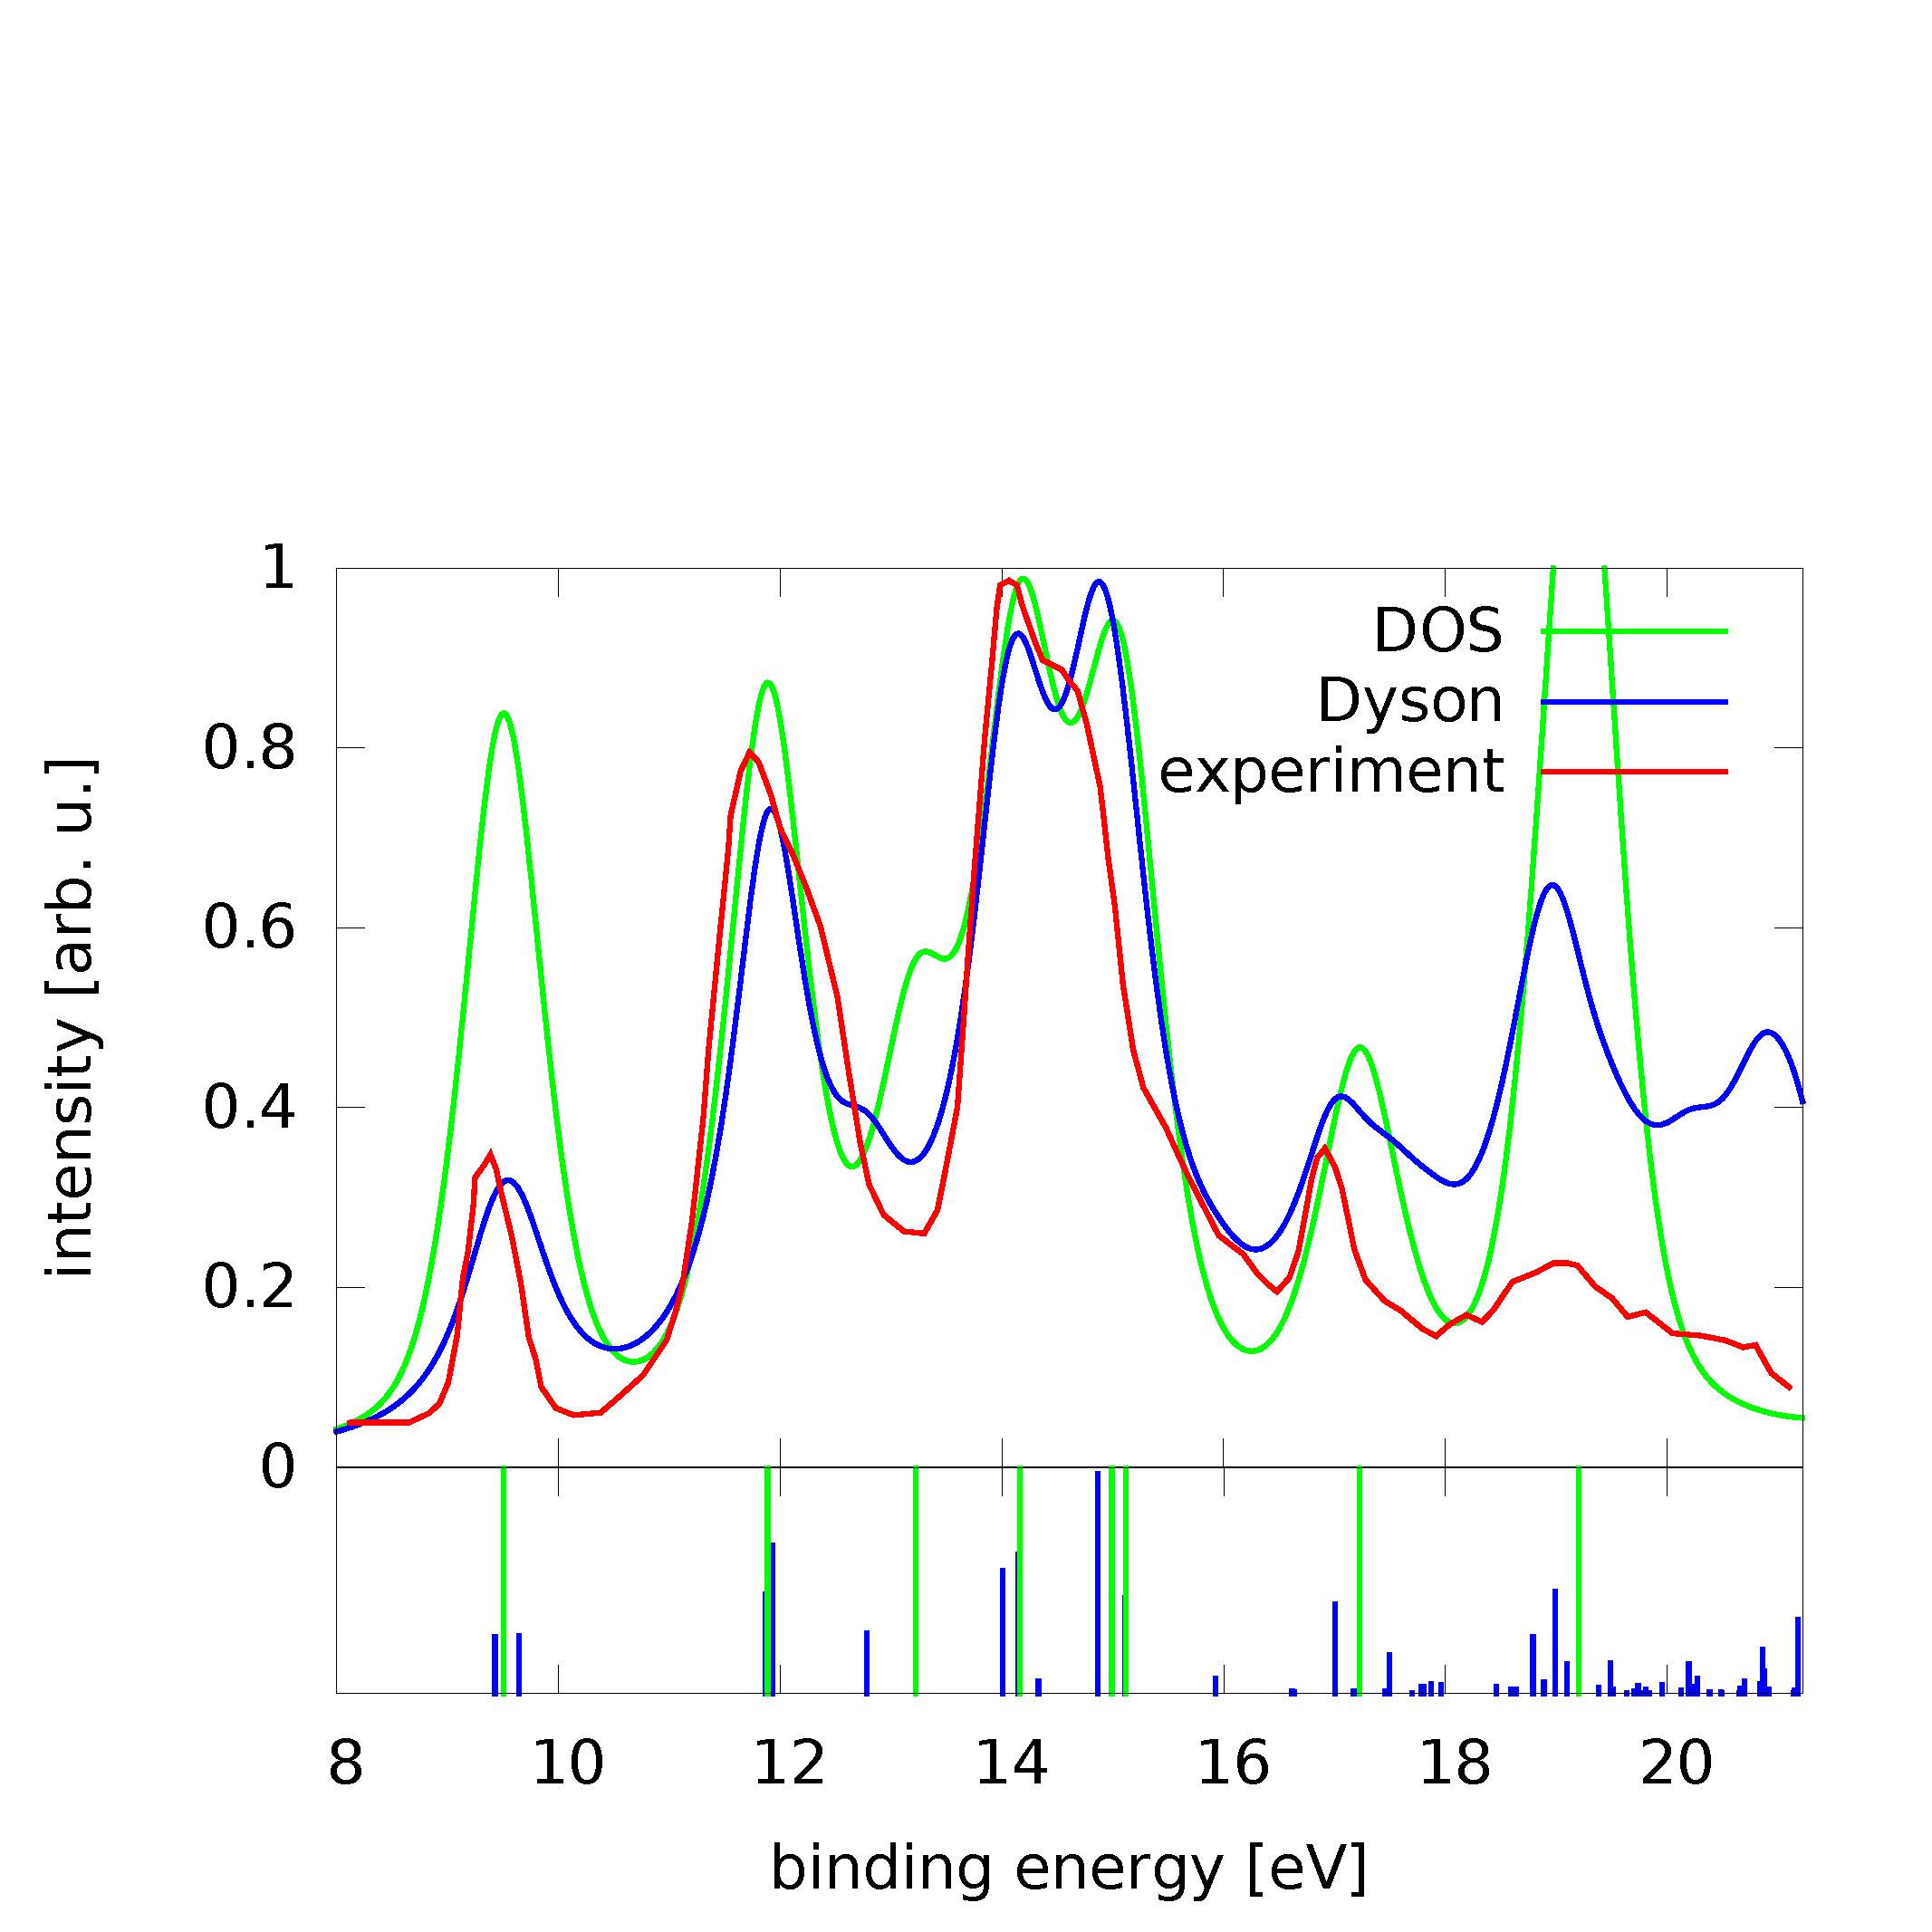
\includegraphics[width=0.5\textwidth]{Figures/Benzene/Benzene}
   \caption{Photoelectron spectra of benzene at different levels of theory.
   In the upper panel the spectra obtained with the Dyson orbital formalism (Dyson) and using the Koopmans' approach (DOS) are compared, the experimental reference is shown in the lower panel \cite{BenzExp}.}
   \label{fig:benzPES}
\end{figure}
%\end{wrapfigure}
The expansion of Coulomb waves includes the terms up to an angular momentum of $l=10$.
The second spectrum shown in 
To indicate the consequences of the OTRSH procedure, in Figure \ref{fig:blypPES} the PES of benzene as predicted with the optimised functional and the B3LYP functional are shown.
For this system, the agreement is good, for other systems the differences are much larger as the example of S$_8$ in the supplement shows.
\begin{figure}
   \includegraphics[width=0.8\textwidth]{Figures/CO2/CO2_spect}
   \caption{I forgot about this degeneracy!!!!!!!}
\end{figure}
\textcolor{red}{
OTRSH is known no be not very good for linear molecules --> is there some reason for this?
}
